\section{研究の目的}
% s0/r0 にフォーカスした話をする.
\begin{frame}
  \frametitle{研究の目的}

  \begin{block}{\textbf{表現力}と\textbf{安全性}を兼ね備えたコード生成言語の構築}
    \begin{itemize}
    \item 表現力: 多段階let挿入,メモ化等の技法を表現
    \item 安全性: 生成されるコードの一定の性質を静的に検査
    \end{itemize}
  \end{block}

  \medskip
  \pause
  % 文字は減らしたほうが良さそう よりってのは何に比べて?
  \begin{block}{本研究: 簡潔で強力なコントロールオペレータに基づくコード生成体系の構築}
    \begin{itemize}
    \item コントロールオペレータ shift0/reset0 を利用し,let挿入などのコード生成技法を表現
    \item 型システムを構築して型安全性を保証
    \end{itemize}
  \end{block}
\end{frame}

\section{研究の内容}
\subsection{本研究の手法}
\begin{frame}
  % 須藤さんの
  \frametitle{本研究の手法}
  % \begin{itemize}
  % \item shift0/reset0 の型システムを単純化; let挿入等に絞る
  % \item これをコード生成言語の型システムに融合
  % \item 型システムの安全性を保証: Kameyama+ 2009, Sudo+2014 の手法を利用
  % \end{itemize}
  \begin{columns}
    \begin{column}{1.\textwidth}%% [横幅] 0.2\textwidth = ページ幅の 20 %
      \center
      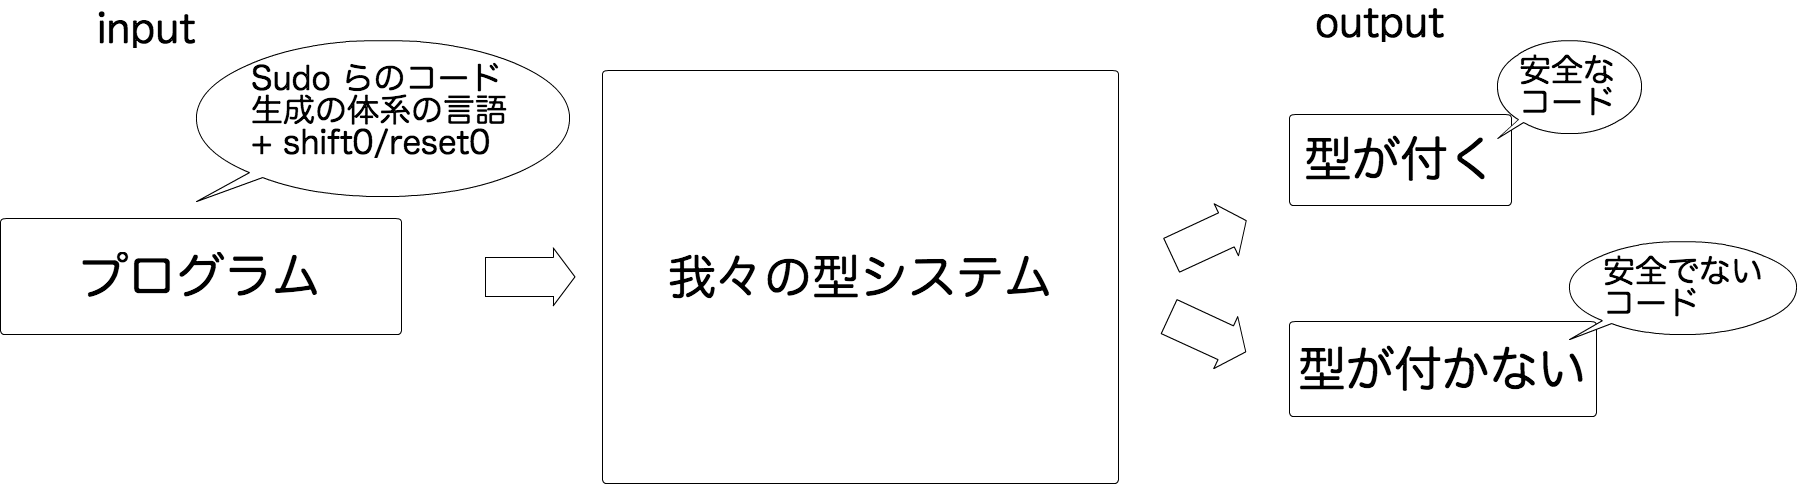
\includegraphics[clip,height=3.2cm]{./img/code_s0r0.png}
    \end{column}
  \end{columns}
\end{frame}

\subsection{コード生成器と生成されるコード}
\begin{frame}
  \frametitle{コード生成器と生成されるコード}
  \begin{onlyenv}<1>
    \begin{columns}
      \begin{column}{0.5\textwidth}%% [横幅] 0.2\textwidth = ページ幅の 20 %
        コード生成器
        \begin{align*}
          & \cforin{i = 0}{n} \\
          & ~~\cforin{j = 0}{m} \\
          & ~~~~\magenta{\cLet~y=t~\cIn} \\
          & ~~~~~~(a\cArrays{i}{j} = b\cArray{i} + y)
        \end{align*}
      \end{column}
      $\Rightarrow$
      \begin{column}{0.5\textwidth}%% [横幅] 0.2\textwidth = ページ幅の 20 %
        生成されるコード
        \begin{align*}
          & \forin{i = 0}{n} \\
          & ~~\forin{j = 0}{m} \\
          & ~~~~\magenta{\Let ~y ~= ~t ~\In} \\
          & ~~~~~~a[i][j] = b[i] + y \\
        \end{align*}
      \end{column}
    \end{columns}
  \end{onlyenv}

  \begin{onlyenv}<2>
    \begin{columns}
      \begin{column}{0.5\textwidth}%% [横幅] 0.2\textwidth = ページ幅の 20 %
        コード生成器
        \begin{align*}
          & \red{...}~ \cforin{i = 0}{n} \\
          & ~~\red{...}~ \cforin{j = 0}{m} \\
          & ~~~~\red{...}~ \magenta{\cLet~y=t~\cIn} \\
          & ~~~~~~\red{...}~ (a\cArrays{i}{j} = b\cArray{i} + y)
        \end{align*}
      \end{column}
      $\Rightarrow$
      \begin{column}{0.5\textwidth}%% [横幅] 0.2\textwidth = ページ幅の 20 %
        生成されるコード
        \begin{align*}
          & \magenta{\Let ~y ~= ~t ~\In} \\
          & ~~\forin{i = 0}{n} \\
          & ~~~~\forin{j = 0}{m} \\
          & ~~~~~~a[i][j] = b[i] + y \\
        \end{align*}
      \end{column}
    \end{columns}
  \end{onlyenv}
\end{frame}


% 以降はコード生成器のみの話にしぼって話します

\subsection{多段階let 挿入}

\begin{frame}
  \frametitle{shift0/reset0 による多段階let挿入}
  \begin{onlyenv}<1>
    コード生成器
    \begin{align*}
      & \red{...}~ \cforin{i = 0}{n} \\
      & ~~\red{...}~ \cforin{j = 0}{m} \\
      & ~~~~\red{...}~ \magenta{\cLet~y=t~\cIn} \\
      & ~~~~~~\red{...}~ (a\cArrays{i}{j} = b\cArray{i} + y)
    \end{align*}
  \end{onlyenv}

  \begin{onlyenv}<2>
    コード生成器
    \begin{align*}
      & \red{\cResetz} ~~\cforin{i = 0}{n} \\
      & ~~\blue{\cResetz} ~~\cforin{j = 0}{m} \\
      & ~~~~\blue{\cShiftz}~\blue{k_2}~\to~ \red{\cShiftz}~\red{k_1}~\to~ \magenta{\cLet~y=t~\cIn} \\
      & ~~~~~~\red{k_1}~(\blue{k_2}~(a\cArrays{i}{j} = b\cArray{i} + y))
    \end{align*}
    \begin{invisibleenv}<2>
      \begin{align*}
        \red{k_1} &= ~~\cforin{i = 0}{n} \\
        \blue{k_2} &= ~~\cforin{j = 0}{m} \\
      \end{align*}
    \end{invisibleenv}
  \end{onlyenv}

  \begin{onlyenv}<3>
    コード生成器
    \begin{align*}
      & \red{\cResetz} ~~\cforin{i = 0}{n} \\
      & ~~\blue{\cResetz} ~~\cforin{j = 0}{m} \\
      & ~~~~\blue{\cShiftz}~\blue{k_2}~\to~ \red{\cShiftz}~\red{k_1}~\to~ \magenta{\cLet~y=t~\cIn} \\
      & ~~~~~~\red{k_1}~(\blue{k_2}~(a\cArrays{i}{j} = b\cArray{i} + y))
    \end{align*}
    \begin{align*}
      \red{k_1} &= ~~\cforin{i = 0}{n} \\
      \blue{k_2} &= ~~\cforin{j = 0}{m} \\
    \end{align*}
  \end{onlyenv}

  \begin{onlyenv}<4>
    コード生成器
    \begin{align*}
      & \magenta{\cLet~y=t~\cIn} \\
      & ~~\red{k_1}~(\blue{k_2}~(a\cArrays{i}{j} = b\cArray{i} + y))
    \end{align*}
    \begin{align*}
      \red{k_1} &= ~~\cforin{i = 0}{n} \\
      \blue{k_2} &= ~~\cforin{j = 0}{m} \\
    \end{align*}
  \end{onlyenv}

  \begin{onlyenv}<5>
    生成されるコード
    \begin{align*}
          & \magenta{\Let ~y ~= ~t ~\In} \\
          & ~~\forin{i = 0}{n} \\
          & ~~~~\forin{j = 0}{m} \\
          & ~~~~~~a[i][j] = b[i] + y \\
    \end{align*}
  \end{onlyenv}
\end{frame}

%%% Local Variables:
%%% mode: japanese-latex
%%% TeX-master: "slide"
%%% End:
